% Options for packages loaded elsewhere
\PassOptionsToPackage{unicode}{hyperref}
\PassOptionsToPackage{hyphens}{url}
%
\documentclass[
  ignorenonframetext,
]{beamer}
\usepackage{pgfpages}
\setbeamertemplate{caption}[numbered]
\setbeamertemplate{caption label separator}{: }
\setbeamercolor{caption name}{fg=normal text.fg}
\beamertemplatenavigationsymbolsempty
% Prevent slide breaks in the middle of a paragraph
\widowpenalties 1 10000
\raggedbottom
\setbeamertemplate{part page}{
  \centering
  \begin{beamercolorbox}[sep=16pt,center]{part title}
    \usebeamerfont{part title}\insertpart\par
  \end{beamercolorbox}
}
\setbeamertemplate{section page}{
  \centering
  \begin{beamercolorbox}[sep=12pt,center]{part title}
    \usebeamerfont{section title}\insertsection\par
  \end{beamercolorbox}
}
\setbeamertemplate{subsection page}{
  \centering
  \begin{beamercolorbox}[sep=8pt,center]{part title}
    \usebeamerfont{subsection title}\insertsubsection\par
  \end{beamercolorbox}
}
\AtBeginPart{
  \frame{\partpage}
}
\AtBeginSection{
  \ifbibliography
  \else
    \frame{\sectionpage}
  \fi
}
\AtBeginSubsection{
  \frame{\subsectionpage}
}
\usepackage{amsmath,amssymb}
\usepackage{lmodern}
\usepackage{iftex}
\ifPDFTeX
  \usepackage[T1]{fontenc}
  \usepackage[utf8]{inputenc}
  \usepackage{textcomp} % provide euro and other symbols
\else % if luatex or xetex
  \usepackage{unicode-math}
  \defaultfontfeatures{Scale=MatchLowercase}
  \defaultfontfeatures[\rmfamily]{Ligatures=TeX,Scale=1}
\fi
\usetheme[]{Ilmenau}
% Use upquote if available, for straight quotes in verbatim environments
\IfFileExists{upquote.sty}{\usepackage{upquote}}{}
\IfFileExists{microtype.sty}{% use microtype if available
  \usepackage[]{microtype}
  \UseMicrotypeSet[protrusion]{basicmath} % disable protrusion for tt fonts
}{}
\makeatletter
\@ifundefined{KOMAClassName}{% if non-KOMA class
  \IfFileExists{parskip.sty}{%
    \usepackage{parskip}
  }{% else
    \setlength{\parindent}{0pt}
    \setlength{\parskip}{6pt plus 2pt minus 1pt}}
}{% if KOMA class
  \KOMAoptions{parskip=half}}
\makeatother
\usepackage{xcolor}
\newif\ifbibliography
\usepackage{color}
\usepackage{fancyvrb}
\newcommand{\VerbBar}{|}
\newcommand{\VERB}{\Verb[commandchars=\\\{\}]}
\DefineVerbatimEnvironment{Highlighting}{Verbatim}{commandchars=\\\{\}}
% Add ',fontsize=\small' for more characters per line
\usepackage{framed}
\definecolor{shadecolor}{RGB}{248,248,248}
\newenvironment{Shaded}{\begin{snugshade}}{\end{snugshade}}
\newcommand{\AlertTok}[1]{\textcolor[rgb]{0.94,0.16,0.16}{#1}}
\newcommand{\AnnotationTok}[1]{\textcolor[rgb]{0.56,0.35,0.01}{\textbf{\textit{#1}}}}
\newcommand{\AttributeTok}[1]{\textcolor[rgb]{0.77,0.63,0.00}{#1}}
\newcommand{\BaseNTok}[1]{\textcolor[rgb]{0.00,0.00,0.81}{#1}}
\newcommand{\BuiltInTok}[1]{#1}
\newcommand{\CharTok}[1]{\textcolor[rgb]{0.31,0.60,0.02}{#1}}
\newcommand{\CommentTok}[1]{\textcolor[rgb]{0.56,0.35,0.01}{\textit{#1}}}
\newcommand{\CommentVarTok}[1]{\textcolor[rgb]{0.56,0.35,0.01}{\textbf{\textit{#1}}}}
\newcommand{\ConstantTok}[1]{\textcolor[rgb]{0.00,0.00,0.00}{#1}}
\newcommand{\ControlFlowTok}[1]{\textcolor[rgb]{0.13,0.29,0.53}{\textbf{#1}}}
\newcommand{\DataTypeTok}[1]{\textcolor[rgb]{0.13,0.29,0.53}{#1}}
\newcommand{\DecValTok}[1]{\textcolor[rgb]{0.00,0.00,0.81}{#1}}
\newcommand{\DocumentationTok}[1]{\textcolor[rgb]{0.56,0.35,0.01}{\textbf{\textit{#1}}}}
\newcommand{\ErrorTok}[1]{\textcolor[rgb]{0.64,0.00,0.00}{\textbf{#1}}}
\newcommand{\ExtensionTok}[1]{#1}
\newcommand{\FloatTok}[1]{\textcolor[rgb]{0.00,0.00,0.81}{#1}}
\newcommand{\FunctionTok}[1]{\textcolor[rgb]{0.00,0.00,0.00}{#1}}
\newcommand{\ImportTok}[1]{#1}
\newcommand{\InformationTok}[1]{\textcolor[rgb]{0.56,0.35,0.01}{\textbf{\textit{#1}}}}
\newcommand{\KeywordTok}[1]{\textcolor[rgb]{0.13,0.29,0.53}{\textbf{#1}}}
\newcommand{\NormalTok}[1]{#1}
\newcommand{\OperatorTok}[1]{\textcolor[rgb]{0.81,0.36,0.00}{\textbf{#1}}}
\newcommand{\OtherTok}[1]{\textcolor[rgb]{0.56,0.35,0.01}{#1}}
\newcommand{\PreprocessorTok}[1]{\textcolor[rgb]{0.56,0.35,0.01}{\textit{#1}}}
\newcommand{\RegionMarkerTok}[1]{#1}
\newcommand{\SpecialCharTok}[1]{\textcolor[rgb]{0.00,0.00,0.00}{#1}}
\newcommand{\SpecialStringTok}[1]{\textcolor[rgb]{0.31,0.60,0.02}{#1}}
\newcommand{\StringTok}[1]{\textcolor[rgb]{0.31,0.60,0.02}{#1}}
\newcommand{\VariableTok}[1]{\textcolor[rgb]{0.00,0.00,0.00}{#1}}
\newcommand{\VerbatimStringTok}[1]{\textcolor[rgb]{0.31,0.60,0.02}{#1}}
\newcommand{\WarningTok}[1]{\textcolor[rgb]{0.56,0.35,0.01}{\textbf{\textit{#1}}}}
\setlength{\emergencystretch}{3em} % prevent overfull lines
\providecommand{\tightlist}{%
  \setlength{\itemsep}{0pt}\setlength{\parskip}{0pt}}
\setcounter{secnumdepth}{-\maxdimen} % remove section numbering
\setbeamertemplate{navigation symbols}{}
\setbeamertemplate{footline}[page number]
\usepackage{amsmath}
\ifLuaTeX
  \usepackage{selnolig}  % disable illegal ligatures
\fi
\IfFileExists{bookmark.sty}{\usepackage{bookmark}}{\usepackage{hyperref}}
\IfFileExists{xurl.sty}{\usepackage{xurl}}{} % add URL line breaks if available
\urlstyle{same} % disable monospaced font for URLs
\hypersetup{
  pdftitle={Multivariate Analysis Lecture 3: Random Vectors and A Random Sample},
  hidelinks,
  pdfcreator={LaTeX via pandoc}}

\title{Multivariate Analysis Lecture 3: Random Vectors and A Random
Sample}
\author{Zhaoxia Yu\\
Professor, Department of Statistics}
\date{2023-04-12}

\begin{document}
\frame{\titlepage}

\hypertarget{review-random-variables-univariate-and-a-random-sample}{%
\section{Review: Random Variables (Univariate) and A Random
Sample}\label{review-random-variables-univariate-and-a-random-sample}}

\hypertarget{random-variables}{%
\subsection{Random Variables}\label{random-variables}}

\begin{frame}{What Is a Random Variable?}
\protect\hypertarget{what-is-a-random-variable}{}
\begin{itemize}
\item
  A random variable is a numerical quantity that takes on different
  values with certain probabilities.
\item
  e.g., a normal distributed random variable takes values between
  \(-\infty\) to \(\infty\).
\item
  It represents the outcome of a random event or experiment.
\item
  e.g., the BMI of a randomly chosen adult living in Canada
\item
  Random variables can be discrete or continuous.
\end{itemize}
\end{frame}

\begin{frame}{The Mean of a Random Variable}
\protect\hypertarget{the-mean-of-a-random-variable}{}
\begin{itemize}
\tightlist
\item
  The mean of a random variable \(X\) measures its central tendency,
  often denoted by \(\mu\) or \(E(X)\).
\item
  It is the expected value of the random variable, weighted by the
  probabilities of each possible outcome:

  \begin{itemize}
  \tightlist
  \item
    Continuous:
    \(\mu = E(X)\overset{def}= \int_{-\infty}^{\infty} x f(x) dx\)
  \item
    Discrete: \(\mu = E(X)\overset{def}= \sum_{i=1}^{} x_i p_i\)
  \end{itemize}
\item
  \(E(aX+b)=aE(X)+b\), where \(X\) is random and \(a\) and \(b\) are
  fixed.
\end{itemize}
\end{frame}

\begin{frame}{Variance of a Random Variable}
\protect\hypertarget{variance-of-a-random-variable}{}
\begin{itemize}
\tightlist
\item
  The variance of a random variable is a measure of how spread out its
  values are around the mean.
\item
  It represents the expected value of the squared deviation of the
  random variable from its mean.
  \(\sigma^2 \overset{def} = E[(X-\mu)^2]\), specifically,

  \begin{itemize}
  \tightlist
  \item
    Continuous:
    \(\sigma^2 \overset{def}= \int_{-\infty}^{\infty} (x - \mu)^2 f(x) dx\)
  \item
    Discrete:
    \(\sigma^2 \overset{def}= \sum_{i=1}^{} (x_i - \mu)^2 p_i\)
  \end{itemize}
\item
  \(\sigma\), the square root of the variance, is called the standard
  deviation (SD) of \(X\).
\end{itemize}
\end{frame}

\begin{frame}{Properties of Variance}
\protect\hypertarget{properties-of-variance}{}
\begin{itemize}
\tightlist
\item
  The variance is a non-negative quantity.
\item
  The variance of a constant is 0: Var(c) = 0, where c is a constant.
\item
  The variance is affected by changes in the scale of the random
  variable but not by a shift in locations: \(Var(aX+b) = a^2 Var(X)\),
  where a is a constant.
\item
  The variance of a sum of \textcolor{red}{independent} random variables
  is the sum of their individual variances:
  \(Var(X + Y) = Var(X) + Var(Y)\), provided that \(X\) and \(Y\) are
  independent.More general, if \(X_1,\cdots, X_n\) are mutually
  independent, then \(Var(\sum_{i=1}^n X_i)=\sum_{i=1}^n Var(X_i)\).
\end{itemize}
\end{frame}

\hypertarget{a-random-sample-of-random-variables}{%
\subsection{A Random Sample of Random
Variables}\label{a-random-sample-of-random-variables}}

\begin{frame}{Random Samples (from Simple Random Sampling)}
\protect\hypertarget{random-samples-from-simple-random-sampling}{}
\begin{itemize}
\tightlist
\item
  In a simple random sample, each member of the population is selected
  independently and with equal probability.
\item
  Obtaining a truly random sample can often be challenging. Reasons:

  \begin{itemize}
  \tightlist
  \item
    it may be difficult or impossible to obtain a complete list of all
    members of the population of interest.
  \item
    it may be costly or time-consuming to sample from the entire
    population.
  \item
    there may be practical constraints on the sampling process, such as
    geographic distance, language barriers, or legal restrictions.
  \item
    certain subgroups of the population may be underrepresented or
    difficult to reach, leading to potential biases in the sample.
  \end{itemize}
\item
  Nevertheless, we assume the samples are simple random samples for
  theoretical derivations
\end{itemize}
\end{frame}

\begin{frame}{Sample Mean and Variance from a Simple Random Samples}
\protect\hypertarget{sample-mean-and-variance-from-a-simple-random-samples}{}
\begin{itemize}
\item
  Let \((X_1, \cdots, X_n)\) be a simple random sample from a
  distribution with mean \(\mu\) and variance \(\sigma^2\). The notation
  we will use is \[X_1, \cdots, X_n \overset{iid}\sim (\mu, \sigma^2)\]
\item
  Summary Statistics and their Expectations:

  \begin{itemize}
  \tightlist
  \item
    The sample mean \(\bar X\) is defined as
    \(\bar X\overset{def}=\frac{1}{n}\sum_{i=1}^n X_i\).
  \item
    \(\bar X\) is unbiased for \(\mu\), i.e., \(E(\bar X)=\mu\).
    \(Var(\bar X)=\sigma^2/n\).
  \item
    The sample variance
    \(S^2\overset{def}=\frac{1}{n-1}\sum_{i=1}^n (X_i-\bar X)^2\).
  \item
    \(S^2\) is unbiased for \(\sigma^2\), i.e., \(E(S^2)=\sigma^2\).
  \end{itemize}
\end{itemize}
\end{frame}

\begin{frame}{Sample Mean is Unbiased}
\protect\hypertarget{sample-mean-is-unbiased}{}
\begin{itemize}
\item
  The proof of unbiasedness follows from the linearity of the expected
  value operator: \[\begin{aligned}
  E(\bar{X}) &= E \left(\frac{1}{n} \sum_{i=1}^{n} X_i \right) 
  = \frac{1}{n} \sum_{i=1}^{n} E(X_i)
  = \frac{1}{n} \sum_{i=1}^{n} \mu
  = \mu
  \end{aligned}\]
\item
  The unbiasedness of the sample mean is a fundamental property of
  statistical estimation.
\end{itemize}
\end{frame}

\begin{frame}{The Variance of the Sample Mean}
\protect\hypertarget{the-variance-of-the-sample-mean}{}
\[\begin{aligned}
Var(\bar{X}) &= Var \left(\frac{1}{n} \sum_{i=1}^{n} X_i \right) 
= \frac{1}{n^2} Var \left(\sum_{i=1}^{n} X_i \right)\\
&= \frac{1}{n^2} \sum_{i=1}^{n} Var(X_i)
= \frac{1}{n^2} \sum_{i=1}^{n} \sigma^2
= \frac{\sigma^2}{n}
\end{aligned}\]

\begin{itemize}
\tightlist
\item
  The variability of the sample means decreases as the sample size
  increases.
\item
  The result is important for the design of experiments and surveys.
  E.g., what is a minimum sample size to achieve a desired level of
  precision?
\end{itemize}
\end{frame}

\begin{frame}{Sample Variance is Unbiased}
\protect\hypertarget{sample-variance-is-unbiased}{}
\begin{itemize}
\tightlist
\item
  The proof of unbiasedness follows from the properties of the variance
  operator and the linearity of the expected value operator:
  \[\begin{aligned}
  E(S^2) &= \frac{1}{n-1} \sum_{i=1}^{n} E[(X_i - \bar{X})^2]
  = \frac{1}{n-1} \sum_{i=1}^{n} E[(X_i - \mu + \mu - \bar{X})^2\\
  &= \frac{1}{n-1} \sum_{i=1}^{n} E[(X_i - \mu)^2 +2(X_i - \mu)(\mu - \bar{X}) + (\mu - \bar{X})^2 ]\\
  &= \frac{1}{n-1} [n \sigma^2 - 2nE[(\mu - \bar{X})^2] + nE[(\mu - \bar{X})^2]]\\
  &= \frac{1}{n-1} (n-1)\sigma^2 = \sigma^2
  \end{aligned}
  \]
\end{itemize}
\end{frame}

\hypertarget{random-vectors-multivariate-and-a-random-sample}{%
\section{Random Vectors (Multivariate) and A Random
Sample}\label{random-vectors-multivariate-and-a-random-sample}}

\hypertarget{random-vectors}{%
\subsection{Random Vectors}\label{random-vectors}}

\begin{frame}{Notations for Random \textcolor{red}{Vectors}}
\protect\hypertarget{notations-for-random}{}
\begin{itemize}
\tightlist
\item
  A random vector is a vector whose elements are random variables. e.g.,
  \[\mathbf{X} = \begin{pmatrix} X_1\\ X_2\\ X_3\end{pmatrix}\] where
  each \(X_i\) is a random variable
\end{itemize}
\end{frame}

\begin{frame}{The Expectation of A Random \textcolor{red}{Vector}}
\protect\hypertarget{the-expectation-of-a-random}{}
\begin{itemize}
\tightlist
\item
  Let \(E(\mathbf{X})\) denote the mean vector of
  \(\mathbf{X}_{p\times 1}\). We have
\end{itemize}

\[\boldsymbol \mu=E(\mathbf{X})\overset{def}=\begin{pmatrix}\mu_1\\ \vdots \\\mu_p \end{pmatrix}, \]
where \(\mu_i=E(X_i), i=1, \cdots, p\).

\begin{itemize}
\tightlist
\item
  Suppose \(X_1, \cdots, X_n \overset{iid} \sim (\mu, \sigma^2)\), and
  \(\mathbf X = (X_1, \cdots, X_n)^T\). What is \(E(\mathbf X)\)?
  \[E(\mathbf X)=E[\begin{pmatrix} X_1 \\ \vdots \\ X_n
  \end{pmatrix}] =
  \begin{pmatrix} \mu \\ \vdots\\ \mu \end{pmatrix}= \mu \mathbf 1\]
\end{itemize}
\end{frame}

\begin{frame}{The Variance-Covariance of A Random Vector}
\protect\hypertarget{the-variance-covariance-of-a-random-vector}{}
\begin{itemize}
\tightlist
\item
  The variance-covariance matrix of a random vector X is a square matrix
  that summarizes the variability and dependence among its components.
\item
  It is denoted by the symbol \(Var(\mathbf X)\), \(Cov(\mathbf X)\), or
  \(\Sigma\) and is given by:
\end{itemize}

\[\begin{aligned}
\Sigma &\overset{def} = E[(\mathbf X - \boldsymbol \mu)(\mathbf X - \boldsymbol \mu)^T]\\
&=
\begin{bmatrix} 
Var(X_1) & Cov(X_1, X_2) & \cdots & Cov(X_1, X_p) \\ 
Cov(X_2, X_1) & Var(X_2) & \cdots & Cov(X_2, X_p) \\
\vdots & \vdots & \ddots & \vdots \\ 
Cov(X_p, X_1) & Cov(X_n, X_2) & \cdots & Var(X_p) 
\end{bmatrix}
\end{aligned}\]
\end{frame}

\begin{frame}{The Variance-Covariance of A Random Vector}
\protect\hypertarget{the-variance-covariance-of-a-random-vector-1}{}
\begin{itemize}
\item
  Alternative notations \[\begin{aligned}
  Var(\mathbf{X}) &= \Sigma = \left(\sigma_{ij}\right)  \overset{def}= 
  \begin{bmatrix} 
  \sigma_1^2 & \sigma_{12} & \cdots & \sigma_{1p} \\ 
  \sigma_{21} & \sigma_2^2 & \cdots & \sigma_{2p} \\
  \vdots & \vdots & \ddots & \vdots \\ 
  \sigma_{p1} & \sigma_{p2} & \cdots & \sigma_p^2 
  \end{bmatrix}
  \end{aligned}\]
\item
  Remarks

  \begin{itemize}
  \tightlist
  \item
    The covariance between two components measures how much they vary
    together, and it can be positive, negative, or zero.
  \item
    \(\Sigma\) is a symmetric matrix because
    \(\sigma_{ij}=Cov(X_i, X_j)=\sigma_{ji}\).
  \item
    The diagonal elements of \(\Sigma\) represent the variances of the
    components of the random vector:
    \(\sigma_i^2=Var(X_i)=Cov(X_i, X_i)\).
  \end{itemize}
\end{itemize}
\end{frame}

\begin{frame}{Correlation Matrix}
\protect\hypertarget{correlation-matrix}{}
\begin{itemize}
\tightlist
\item
  A correlation matrix is a table showing correlation coefficients
  between different variables.
\item
  The correlation coefficient measures the strength and direction of the
  linear relationship between two variables. \[
  \text{Corr}(X_i,X_j)=\frac{\text{Cov}(X_i,X_j)}{\sqrt{Var(X_i)}\sqrt{Var(X_j)}}=\frac{\sigma_{ij}}{\sigma_i \sigma_j}
  \]
\item
  The correlation coefficient ranges from -1 to 1, with values close to
  -1 indicating a strong negative linear relationship, values close to 1
  indicating a strong positive linear relationship, and values close to
  0 indicating no linear relationship.
\end{itemize}
\end{frame}

\begin{frame}{Correlation Matrix}
\protect\hypertarget{correlation-matrix-1}{}
\[
\mathbf{R} = \begin{bmatrix} 1 & \text{Corr}(X_1,X_2) & \cdots & \text{Corr}(X_1,X_p) \\ \text{Corr}(X_2,X_1) & 1 & \cdots & \text{Corr}(X_2,X_p) \\ \vdots & \vdots & \ddots & \vdots \\ \text{Corr}(X_p,X_1) & \text{Corr}(X_p,X_2) & \cdots & 1 \end{bmatrix}
\] - \(\rho_{ij}\overset{def}=Corr(X_i, X_j)\) - The diagonal
\(\rho_{ii}\) of the correlation matrix shows the correlation of each
variable with itself, which is always equal to 1. - The matrix is
symmetric since the correlation between X and Y is the same as the
correlation between Y and X: \(\rho_{ij}=\rho_{ji}\). - Correlation
matrix can help identify variables that are correlated.
\end{frame}

\begin{frame}{Covariance Matrix of Two Random Vectors}
\protect\hypertarget{covariance-matrix-of-two-random-vectors}{}
\begin{itemize}
\tightlist
\item
  The covariance matrix of two random vectors
  \(\mathbf{X}=(X_1,\dots,X_p)^T\) and \(\mathbf{Y}=(Y_1,\dots,Y_q)^T\)
  is a \(p\times q\) matrix defined as
\end{itemize}

\[
\begin{aligned}
\mathbf{Cov}(\mathbf{X},\mathbf{Y}) & \overset{def}= E[(\mathbf X-\boldsymbol \mu_X)(\mathbf Y-\boldsymbol \mu_Y)^T]\\
&= \begin{bmatrix} \text{Cov}(X_1,Y_1) & \cdots & \text{Cov}(X_1,Y_q) \\ \vdots & \ddots & \vdots \\ \text{Cov}(X_p,Y_1) & \cdots & \text{Cov}(X_p,Y_q) \end{bmatrix}
\end{aligned}
\]

\begin{itemize}
\tightlist
\item
  Each element of the matrix is the covariance between two corresponding
  elements of the vectors.
\end{itemize}
\end{frame}

\begin{frame}{Covariance Matrix of Two Random Vectors}
\protect\hypertarget{covariance-matrix-of-two-random-vectors-1}{}
\begin{itemize}
\tightlist
\item
  E.g.,
  \[\mathbf X_{2\times 1}=\begin{pmatrix}X_1 & X_2\end{pmatrix}^T, \mathbf Y_{3\times 1}=\begin{pmatrix}Y_1 & Y_2 & Y_3\end{pmatrix}\]
  \[
  \begin{aligned}
  &Cov(\mathbf X,\mathbf Y)&=E[(X-E(X))(Y-E(Y))^T]\\
  =&E[\begin{pmatrix}X_1 -\mu_{x1} \\ X_2- \mu_{x2}\end{pmatrix}
  (Y_1-\mu_{y1}, Y_2 -\mu_{y2}, Y_3-\mu_{y3})^T]\\
  =&\begin{bmatrix} 
  E[(X_1 -\mu_{x1})(Y_1 -\mu_{y1})] &E[(X_1 -\mu_{x1})(Y_2 -\mu_{y2})]  &E[(X_1 -\mu_{x1})(Y_3 -\mu_{y3})] \\
  E[(X_2 -\mu_{x2})(Y_1 -\mu_{y1})] &E[(X_2 -\mu_{x2})(Y_2 -\mu_{y2})]  &E[(X_3 -\mu_{x3})(Y_3 -\mu_{y3})]\end{bmatrix}\\
  =&\begin{bmatrix} 
  Cov(X_1, Y_1) & Cov(X_1, Y_2) & Cov(X_1, Y_3)\\
  Cov(X_2, Y_1) & Cov(X_2, Y_2) & Cov(X_2, Y_3)
  \end{bmatrix}
  \end{aligned}\]
\item
  Note:
  \(\mathbf{Cov}(\mathbf{X},\mathbf{Y}) = [\mathbf{Cov}(\mathbf{Y},\mathbf{X})]^T\)
\end{itemize}
\end{frame}

\hypertarget{a-random-sample-of-random-vectors}{%
\subsection{A Random Sample of Random
Vectors}\label{a-random-sample-of-random-vectors}}

\begin{frame}{Notations about A Random Sample of Random Vectors}
\protect\hypertarget{notations-about-a-random-sample-of-random-vectors}{}
\begin{itemize}
\item
  Consider a random sample from a \textcolor{red}{multivariate}
  distribution with mean vector \(\boldsymbol \mu_{p\times 1}\) and
  covariance \(\boldsymbol \Sigma_{p\times p}\)
\item
  A random sample of random vectors is a collection of \(n\) independent
  and identically distributed random vectors, denoted as
  \(\mathbf{X}_1, \mathbf{X}_2, \dots, \mathbf{X}_n\).
\item
  The random sample of random vectors is denoted by
  \[\mathbf X_{n\times p} = \begin{pmatrix}\mathbf X_1^T \\ \vdots \\ \mathbf X_n^T\end{pmatrix}\]
\item
  Each random vector \(\mathbf{X}_i\) is of dimension \(p\) and can be
  represented as: \[
  \mathbf{X}_i = (X_{i1}, X_{i2}, \dots, X_{ip})^T
  \]
\end{itemize}
\end{frame}

\begin{frame}{Sample Mean Vector \(\bar{\mathbf{X}}_{p\times 1}\)}
\protect\hypertarget{sample-mean-vector-barmathbfx_ptimes-1}{}
\begin{itemize}
\tightlist
\item
  The sample mean vector, denoted as \(\bar{\mathbf{X}}\), is a random
  vector of dimension \(p\), defined as: \[
  \bar{\mathbf{X}} = \frac{1}{n}\sum_{i=1}^n \mathbf{X}_i
  \]
\item
  It is unbiased for the population mean vector \(\boldsymbol \mu\)
  because
  \[E[\bar{\mathbf{X}}] = E[\frac{1}{n}\sum_{i=1}^n \mathbf{X}_i]= \frac{1}{n}\sum_{i=1}^n E[\mathbf{X}_i] =\frac{1}{n}\sum_{i=1}^n \boldsymbol \mu =\boldsymbol \mu\]
\item
  The sample mean vector \(\bar{\mathbf{X}}\) is often used to estimate
  the population mean vector \(\boldsymbol \mu\).
\end{itemize}
\end{frame}

\begin{frame}{The Covariance of the Sample Mean Vector}
\protect\hypertarget{the-covariance-of-the-sample-mean-vector}{}
\begin{itemize}
\tightlist
\item
  The sample mean vector, denoted as \(\bar{\mathbf{X}}\), is a random
  vector of dimension \(p\). We can also compute its covariance matrix
\item
  Because \((\mathbf X_1, \cdots, \mathbf X_n)\) are iid ,
  \[Cov(\bar{\mathbf{X}}) = Cov(\frac{1}{n}\sum_{i=1}^n \mathbf{X}_i)= \frac{1}{n^2}\sum_{i=1}^n Cov(\mathbf{X}_i)=\frac{1}{n}\boldsymbol \Sigma\]
\item
  Similar to the population mean vector, the population covariance
  \(\boldsymbol \Sigma\) is typically unknown. If we have a random
  sample, we can estimate it - the sample covariance matrix.S
\end{itemize}
\end{frame}

\begin{frame}{Sample Covariance Matrix \(\mathbf{S}_{p\times p}\)}
\protect\hypertarget{sample-covariance-matrix-mathbfs_ptimes-p}{}
\begin{itemize}
\tightlist
\item
  The sample covariance matrix, denoted as \(\mathbf{S}\), is a
  \(p \times p\) symmetric matrix, defined as:
\end{itemize}

\[
\mathbf{S} = \frac{1}{n-1}\sum_{i=1}^n (\mathbf{X}_i - \bar{\mathbf{X}})(\mathbf{X}_i - \bar{\mathbf{X}})^T
\] - Next, we show that the sample covariance matrix \(\mathbf{S}\) is
an unbiased estimator of \(\boldsymbol{\Sigma}\):

\[
\mathbb{E}[\mathbf{S}] = \boldsymbol{\Sigma}
\]
\end{frame}

\begin{frame}{The Sample Covariance Matrix is Unbiased: Lemmas}
\protect\hypertarget{the-sample-covariance-matrix-is-unbiased-lemmas}{}
\begin{itemize}
\tightlist
\item
  Lemma 1:
  \(E(\mathbf X_i \mathbf X_i^T)= \boldsymbol \mu \boldsymbol \mu^T + Cov(\mathbf X_i)=\boldsymbol \mu \boldsymbol \mu^T + \boldsymbol \Sigma\).
  -Proof. By the definition of Cov, we have \[\begin{aligned}
  \boldsymbol \Sigma &=E[(\mathbf X_i-\boldsymbol \mu)(\mathbf X_i-\boldsymbol \mu)^T] \\
  &= E[\mathbf X_i \mathbf X_i^T - \boldsymbol \mu\mathbf X_i^T - \mathbf X_i \boldsymbol \mu^T + \boldsymbol \mu \boldsymbol \mu^T]\\
  &= E[\mathbf X_i \mathbf X_i^T] - \boldsymbol \mu E[\mathbf X_i^T] - E[\mathbf X_i] \boldsymbol \mu^T + \boldsymbol \mu \boldsymbol \mu^T\\
  &= E[\mathbf X_i \mathbf X_i^T] - \boldsymbol \mu \boldsymbol \mu^T - \boldsymbol \mu \boldsymbol \mu^T + \boldsymbol \mu \boldsymbol \mu^T\\
  &= E[\mathbf X_i \mathbf X_i^T] - \boldsymbol \mu \boldsymbol \mu^T
  \end{aligned}\] As a result,
  \(E[\mathbf X_i \mathbf X_i^T]= \boldsymbol \mu \boldsymbol \mu^T + \boldsymbol \Sigma\).
\item
  Similarly, we have Lemma 2:
  \[E(\bar {\mathbf X} \bar {\mathbf X}^T)=\boldsymbol \mu \boldsymbol \mu^T + Cov(\bar {\mathbf X})=\boldsymbol \mu \boldsymbol \mu^T + \frac{1}{n}\boldsymbol \Sigma\]
\end{itemize}
\end{frame}

\begin{frame}{The Sample Covariance Matrix is Unbiased: Proof}
\protect\hypertarget{the-sample-covariance-matrix-is-unbiased-proof}{}
\begin{itemize}
\item
  Proof:Expand the product:

  \[
  \begin{aligned}
  \mathbf{S} &= \frac{1}{n-1}\sum_{i=1}^n (\mathbf{X}_i \mathbf{X}_i^T - \mathbf{X}_i \bar{\mathbf{X}}^T - \bar{\mathbf{X}} \mathbf{X}_i^T + \bar{\mathbf{X}} \bar{\mathbf{X}}^T) \\
  &=\frac{1}{n-1}[\sum_{i=1}^n \mathbf{X}_i \mathbf{X}_i^T- n\bar{\mathbf X}\bar{\mathbf X}^T 
  -n\bar{\mathbf X}\bar{\mathbf X}^T + n\bar{\mathbf X}\bar{\mathbf X}^T]\\
  &= \frac{1}{n-1}\sum_{i=1}^n \mathbf{X}_i \mathbf{X}_i^T - \frac{n}{n-1}\bar{\mathbf{X}} \bar{\mathbf{X}}^T
  \end{aligned}
  \]
\end{itemize}
\end{frame}

\begin{frame}{The Sample Covariance Matrix is Unbiased: Proof
(continued)}
\protect\hypertarget{the-sample-covariance-matrix-is-unbiased-proof-continued}{}
\begin{itemize}
\tightlist
\item
  Taking the expected value: \[
  \begin{aligned}
  \mathbb{E}[\mathbf{S}] &= \mathbb{E}\left[\frac{1}{n-1}\sum_{i=1}^n \mathbf{X}_i \mathbf{X}_i^T - \frac{n}{n-1}\bar{\mathbf{X}} \bar{\mathbf{X}}^T\right] \\
  &= \frac{1}{n-1}\sum_{i=1}^n \mathbb{E}[\mathbf{X}_i \mathbf{X}_i^T] - \frac{n}{n-1}\mathbb{E}[\bar{\mathbf{X}} \bar{\mathbf{X}}^T] \\
  &= \frac{1}{n-1}\sum_{i=1}^n (\boldsymbol{\Sigma} + \boldsymbol{\mu}\boldsymbol{\mu}^T) - \frac{n}{n-1}(\boldsymbol{\frac{1}{n}\Sigma} + \boldsymbol{\mu}\boldsymbol{\mu}^T) \\
  &= \frac{n}{n-1}\boldsymbol{\Sigma} + \frac{n}{n-1}\boldsymbol{\mu}\boldsymbol{\mu}^T - \frac{1}{n-1}\boldsymbol{\Sigma} - \frac{n}{n-1}\boldsymbol{\mu}\boldsymbol{\mu}^T \\
  &= \boldsymbol{\Sigma}
  \end{aligned}
  \]
\item
  Therefore, the sample covariance matrix is unbiased
\end{itemize}
\end{frame}

\begin{frame}{Examples: The Iris Setosa Data}
\protect\hypertarget{examples-the-iris-setosa-data}{}
\begin{itemize}
\tightlist
\item
  The iris data consists of three random samples, one for each species.
  Consider the setosa sample.
\item
  It is a random sample (let's assume it) of size 50.
\item
  The data matrix has \(n=50\) rows and \(p=4\) columns
\end{itemize}
\end{frame}

\begin{frame}[fragile]{The Data Matrix of Iris Setosa}
\protect\hypertarget{the-data-matrix-of-iris-setosa}{}
\begin{Shaded}
\begin{Highlighting}[]
\NormalTok{setosa}\OtherTok{=}\FunctionTok{as.matrix}\NormalTok{(iris[iris}\SpecialCharTok{$}\NormalTok{Species}\SpecialCharTok{==}\StringTok{"setosa"}\NormalTok{, }\DecValTok{1}\SpecialCharTok{:}\DecValTok{4}\NormalTok{])}
\FunctionTok{dim}\NormalTok{(setosa)}
\end{Highlighting}
\end{Shaded}

\begin{verbatim}
## [1] 50  4
\end{verbatim}

\begin{Shaded}
\begin{Highlighting}[]
\FunctionTok{head}\NormalTok{(setosa)}
\end{Highlighting}
\end{Shaded}

\begin{verbatim}
##   Sepal.Length Sepal.Width Petal.Length Petal.Width
## 1          5.1         3.5          1.4         0.2
## 2          4.9         3.0          1.4         0.2
## 3          4.7         3.2          1.3         0.2
## 4          4.6         3.1          1.5         0.2
## 5          5.0         3.6          1.4         0.2
## 6          5.4         3.9          1.7         0.4
\end{verbatim}
\end{frame}

\begin{frame}[fragile]{The Sample Mean of Iris Setosa}
\protect\hypertarget{the-sample-mean-of-iris-setosa}{}
\begin{Shaded}
\begin{Highlighting}[]
\NormalTok{sample.meanvec}\OtherTok{=}\FunctionTok{matrix}\NormalTok{(}\FunctionTok{colMeans}\NormalTok{(setosa), }\DecValTok{4}\NormalTok{, }\DecValTok{1}\NormalTok{)}
\FunctionTok{rownames}\NormalTok{(sample.meanvec)}\OtherTok{=}\FunctionTok{colnames}\NormalTok{(setosa)}
\FunctionTok{colnames}\NormalTok{(sample.meanvec)}\OtherTok{=}\StringTok{"mean"}
\NormalTok{sample.meanvec}
\end{Highlighting}
\end{Shaded}

\begin{verbatim}
##               mean
## Sepal.Length 5.006
## Sepal.Width  3.428
## Petal.Length 1.462
## Petal.Width  0.246
\end{verbatim}
\end{frame}

\begin{frame}[fragile]{Pairwise Scatter Plot of the Features of Iris
Setosa}
\protect\hypertarget{pairwise-scatter-plot-of-the-features-of-iris-setosa}{}
\begin{Shaded}
\begin{Highlighting}[]
\FunctionTok{scatterplotMatrix}\NormalTok{(setosa)}
\end{Highlighting}
\end{Shaded}

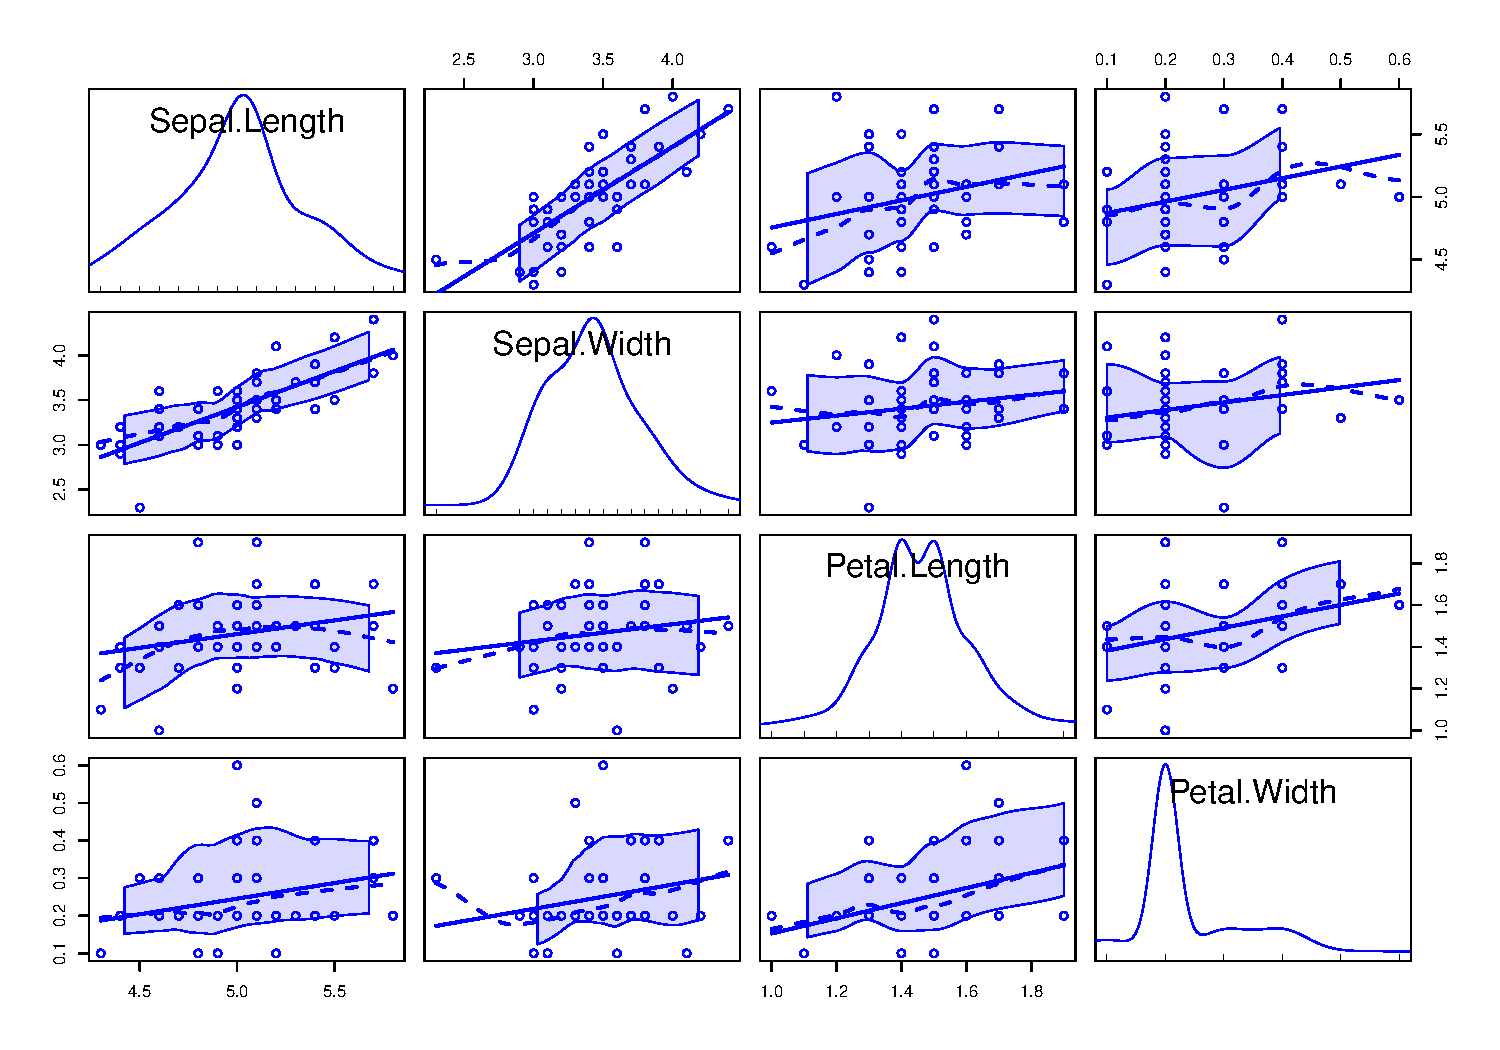
\includegraphics[width=0.75\linewidth]{Lecture03_RandomV_files/figure-beamer/unnamed-chunk-3-1}
\end{frame}

\begin{frame}[fragile]{The Sample Covariane Matrix of Iris Setosa}
\protect\hypertarget{the-sample-covariane-matrix-of-iris-setosa}{}
\begin{Shaded}
\begin{Highlighting}[]
\NormalTok{sample.cov}\OtherTok{=}\FunctionTok{cov}\NormalTok{(setosa)}
\FunctionTok{round}\NormalTok{(sample.cov,}\DecValTok{2}\NormalTok{)}
\end{Highlighting}
\end{Shaded}

\begin{verbatim}
##              Sepal.Length Sepal.Width Petal.Length Petal.Width
## Sepal.Length         0.12        0.10         0.02        0.01
## Sepal.Width          0.10        0.14         0.01        0.01
## Petal.Length         0.02        0.01         0.03        0.01
## Petal.Width          0.01        0.01         0.01        0.01
\end{verbatim}
\end{frame}

\begin{frame}[fragile]{The Sample Correlation Matrix of Iris Setosa}
\protect\hypertarget{the-sample-correlation-matrix-of-iris-setosa}{}
\begin{Shaded}
\begin{Highlighting}[]
\NormalTok{sample.corr}\OtherTok{=}\FunctionTok{cor}\NormalTok{(setosa)}
\FunctionTok{corrplot}\NormalTok{(sample.corr)}
\end{Highlighting}
\end{Shaded}

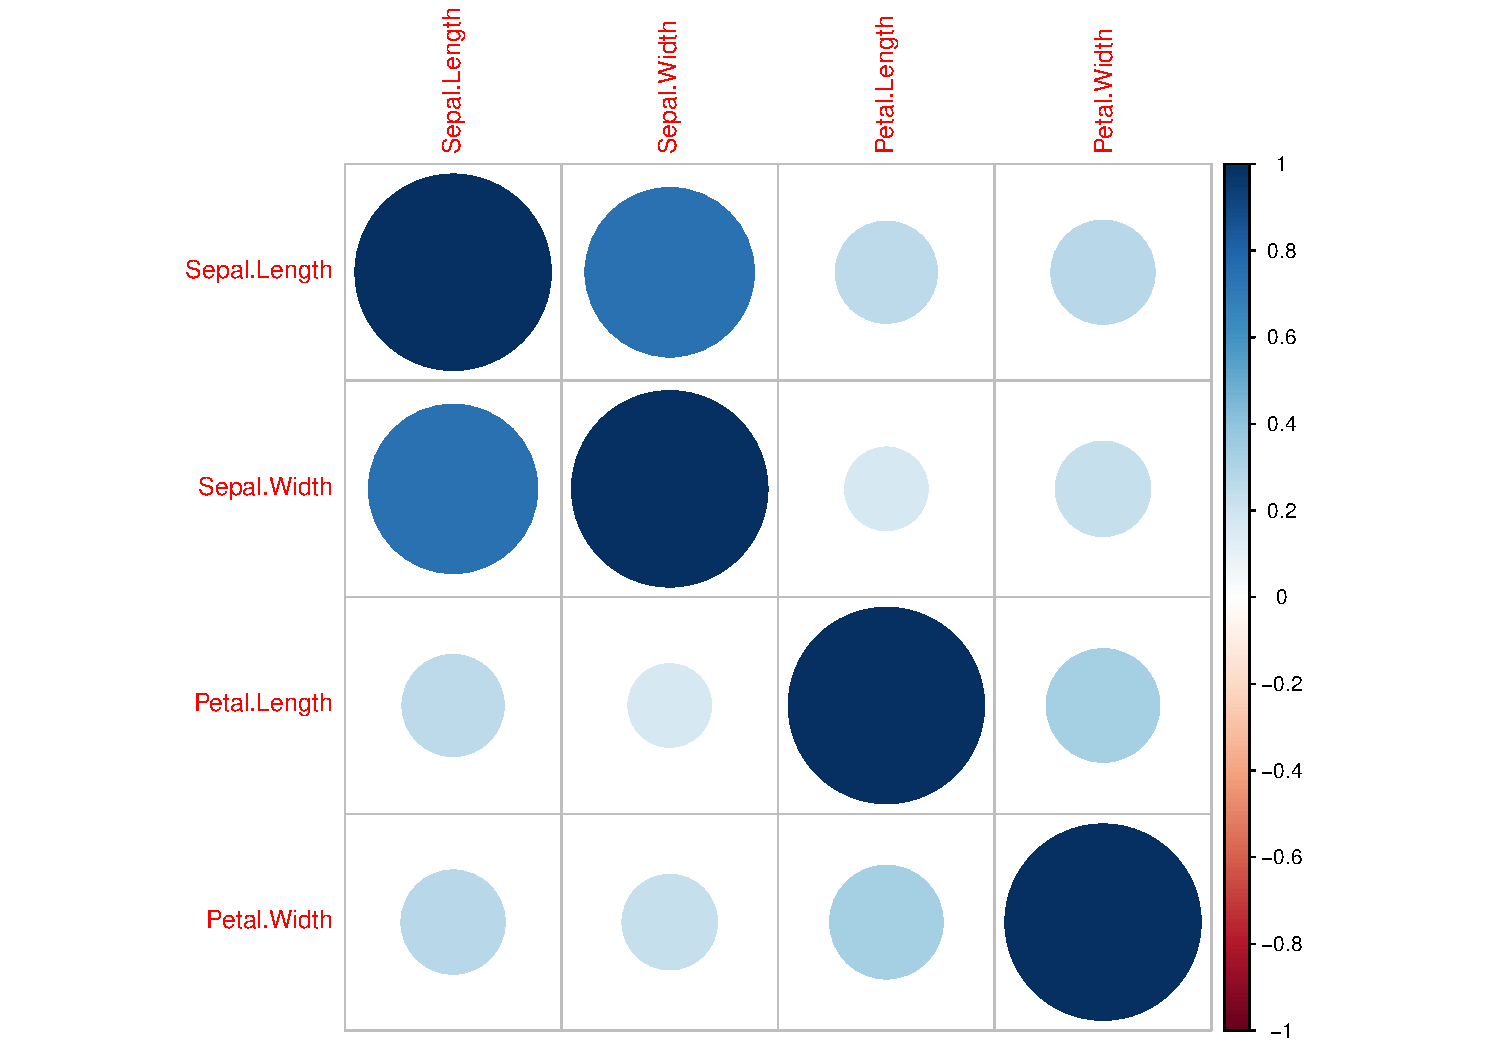
\includegraphics[width=0.8\linewidth]{Lecture03_RandomV_files/figure-beamer/unnamed-chunk-5-1}
\end{frame}

\begin{frame}[fragile]{The Sample Correlation Matrix of Iris Setosa}
\protect\hypertarget{the-sample-correlation-matrix-of-iris-setosa-1}{}
\begin{Shaded}
\begin{Highlighting}[]
\FunctionTok{corrplot}\NormalTok{(sample.corr, }\AttributeTok{method=}\StringTok{"number"}\NormalTok{)}
\end{Highlighting}
\end{Shaded}

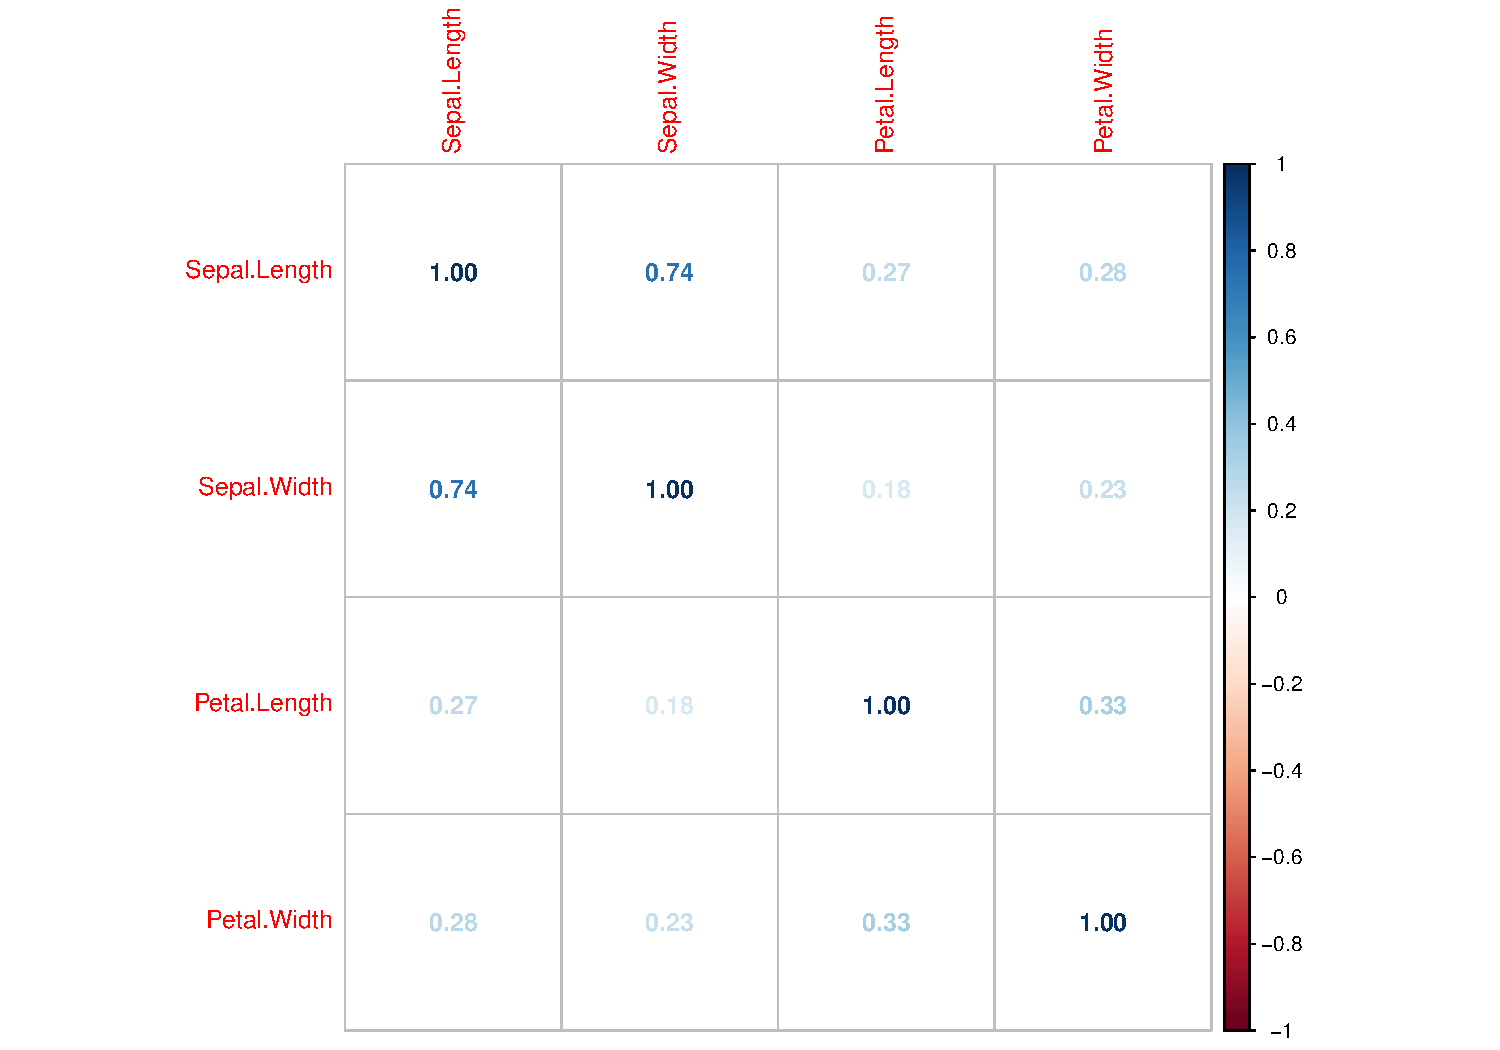
\includegraphics[width=0.8\linewidth]{Lecture03_RandomV_files/figure-beamer/unnamed-chunk-6-1}
\end{frame}

\begin{frame}[fragile]{The Sample Correlation Matrix of Iris Setosa}
\protect\hypertarget{the-sample-correlation-matrix-of-iris-setosa-2}{}
\begin{Shaded}
\begin{Highlighting}[]
\FunctionTok{corrplot}\NormalTok{(sample.corr, }\AttributeTok{method=}\StringTok{"ellipse"}\NormalTok{)}
\end{Highlighting}
\end{Shaded}

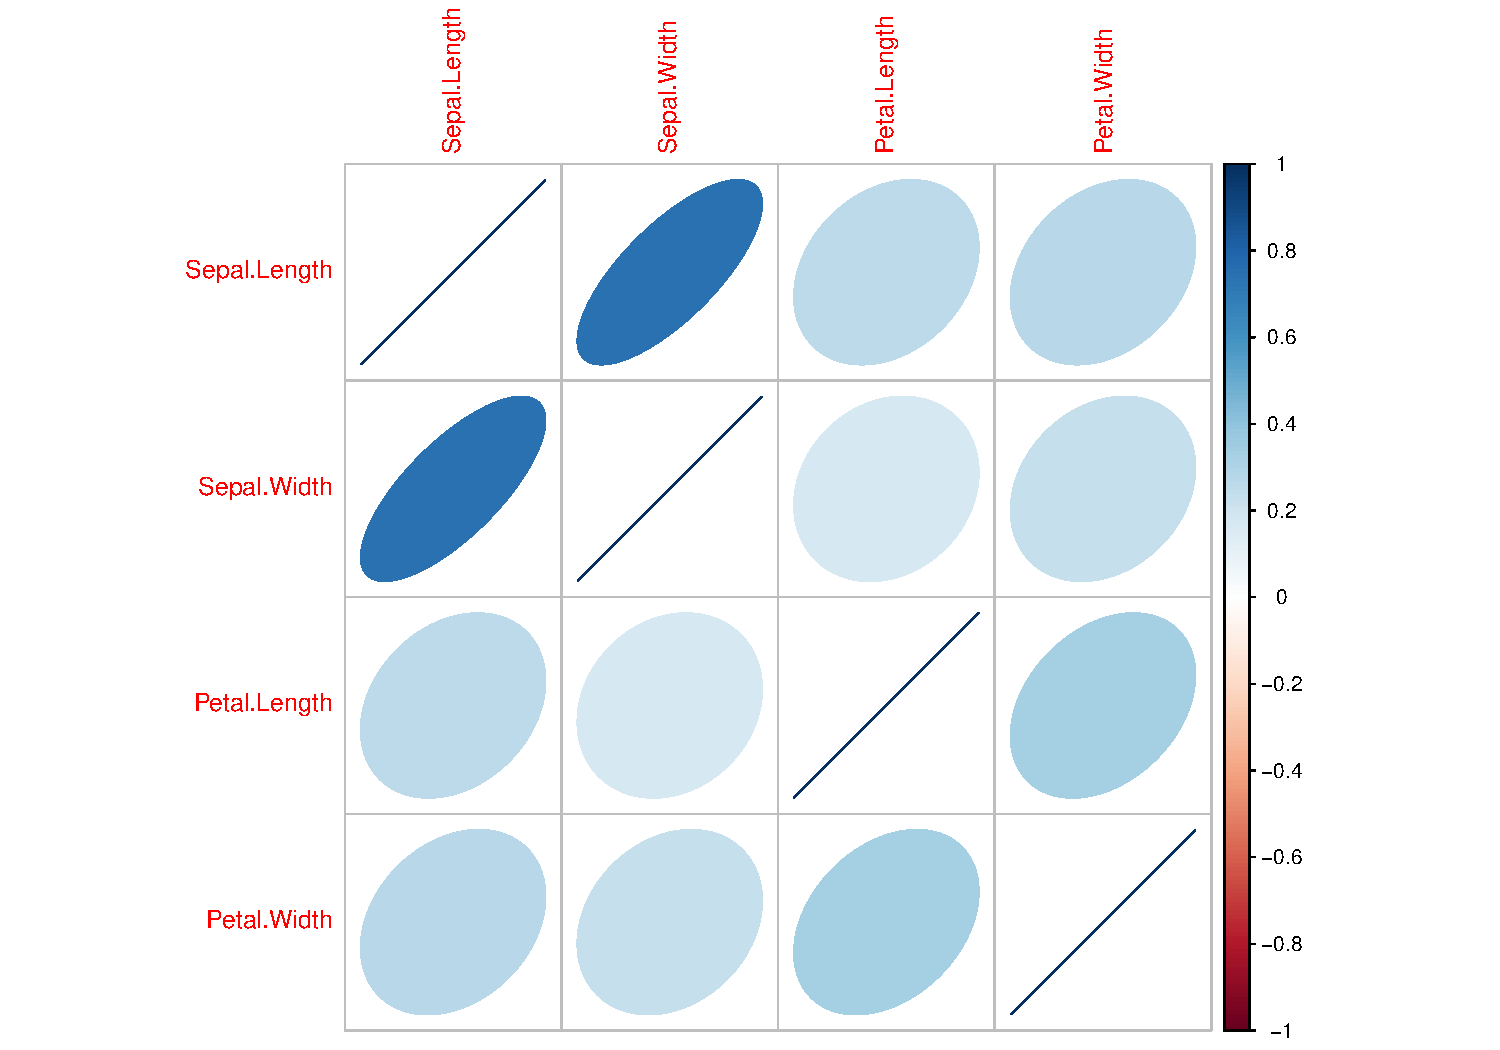
\includegraphics[width=0.8\linewidth]{Lecture03_RandomV_files/figure-beamer/unnamed-chunk-7-1}
\end{frame}

\begin{frame}{Sample Covariate Matrix as a Quadratic Form}
\protect\hypertarget{sample-covariate-matrix-as-a-quadratic-form}{}
\[(n-1)S = \sum (X_i- \bar X) (X_i- \bar X)^T=
\begin{pmatrix}X_1 - \bar X & \cdots X_n -\bar X\end{pmatrix}
\begin{pmatrix}(X_1 - \bar X)^T \\ \vdots \\(X_n - \bar X)^T\end{pmatrix}
\] Note that
\[\begin{pmatrix}(X_1 - \bar X)^T \\ \vdots \\(X_n - \bar X)^T\end{pmatrix}= \begin{pmatrix}X_1 - \bar X \\ \vdots \\ X_n - \bar X\end{pmatrix}^T=\mathbf C\mathbf X\]
where \(\mathbf C\) is the centering matrix defined in assignment 1,
i.e., \(\mathbf C = \mathbf I_n - \frac{1}{n} \mathbf 1 \mathbf 1^T\).
In addition, it can be verified that \(\mathbf C^T\mathbf C=\mathbf C\).

Therefore, \[(n-1)S=(C\mathbf X)^T C\mathbf X= \mathbf X^T C \mathbf X\]
\end{frame}

\hypertarget{linear-combination-of-a-random-vector-yatx}{%
\section{\texorpdfstring{Linear Combination of a Random Vector:
\(Y=a^TX\)}{Linear Combination of a Random Vector: Y=a\^{}TX}}\label{linear-combination-of-a-random-vector-yatx}}

\begin{frame}{Definition of a Linear Combination of a Random Vector}
\protect\hypertarget{definition-of-a-linear-combination-of-a-random-vector}{}
\begin{itemize}
\item
  Let \(\mathbf{X}\) be a \(p\)-dimensional random vector with mean
  vector \(\boldsymbol{\mu}\) and covariance matrix
  \(\boldsymbol{\Sigma}\).
\item
  Consider a linear combination of the form:
  \[  Y = \mathbf{a}^T\mathbf{X}\]

  where \(\mathbf{a}\) is a \(p\)-dimensional constant vector.
\item
  E.g., \(\mathbf X = (X_1, X_2, X_3)^T\), \(a=(1/3, 1/3, 1/3)^T\). Then
  \[Y=a^TX=\frac{1}{3}(X_1 + X_2 + X_3)\]
\end{itemize}
\end{frame}

\begin{frame}{Mean of \(Y=a^TX\)}
\protect\hypertarget{mean-of-yatx}{}
\begin{itemize}
\item
  The mean of \(Y\) can be expressed as: \[
  \begin{aligned}
  E(Y) &= E(\mathbf{a}^T\mathbf{X}) \\
  &= \mathbf{a}^T E(\mathbf{X}) \\
  &= \mathbf{a}^T \boldsymbol{\mu}
  \end{aligned}
  \]
\item
  Intuitively, the mean of \(Y\) is a weighted average of the components
  of \(\mathbf{X}\), with weights given by the corresponding components
  of \(\mathbf{a}\).
\end{itemize}
\end{frame}

\begin{frame}{Variance of \(Y\)}
\protect\hypertarget{variance-of-y}{}
\begin{itemize}
\item
  The variance of \(Y\) can be expressed as: \[
  \begin{aligned}
  \text{Var}(Y) &= \text{Var}(\mathbf{a}^T\mathbf{X}) \\
  &= \mathbf{a}^T \boldsymbol{\Sigma} \mathbf{a}
  \end{aligned}
  \]
\item
  The variance of \(Y\) depends on the covariance structure of
  \(\mathbf{X}\), as well as the weights given by \(\mathbf{a}\). If the
  components of \(\mathbf{a}\) are uncorrelated or orthogonal, then the
  variance of \(Y\) is simply a weighted sum of the variances of the
  components of \(\mathbf{X}\). However, if the components of
  \(\mathbf{a}\) are correlated, then the covariance structure of
  \(\mathbf{X}\) affects the variance of \(Y\) as well.
\end{itemize}
\end{frame}

\begin{frame}{Linear Combinations of Iris Setosa Features}
\protect\hypertarget{linear-combinations-of-iris-setosa-features}{}
\begin{itemize}
\tightlist
\item
  Recall that for the iris setosa, \(\mathbf X\) is \(50\times 4\).
\item
  Consider a linear combination of the features \(Y= Xb\), where \[
  b=\begin{pmatrix}
  1/4 \\ 1/4 \\ 1/4 \\ 1/4
  \end{pmatrix}\]
\item
  \(Yb\) is a \(50\times 1\) vector, with the \(i\)th row be the average
  of the four features of the \(i\)th iris setosa flower. To see this
\end{itemize}
\end{frame}

\begin{frame}[fragile]{Linear Combinations of Iris Setosa Features}
\protect\hypertarget{linear-combinations-of-iris-setosa-features-1}{}
\[\begin{aligned}
Y&=Xb=
\begin{pmatrix} X_1^T \\ \vdots \\ X_n^T  \end{pmatrix} b
 =
\begin{pmatrix} X_1^Tb \\ \vdots \\ X_n^Tb  \end{pmatrix}
=\begin{pmatrix} \frac{x_{11} +x_{12} + x_{13} + x_{14}}{4}  \\ 
\vdots \\ 
 \frac{x_{n1} +x_{n2} + x_{n3} + x_{n4}}{4}   \end{pmatrix}
\end{aligned}
\] \#\#\# Linear Combinations of Iris Setosa Features: sample mean

\begin{Shaded}
\begin{Highlighting}[]
\NormalTok{b}\OtherTok{=}\FunctionTok{matrix}\NormalTok{(}\DecValTok{1}\SpecialCharTok{/}\DecValTok{4}\NormalTok{, }\DecValTok{4}\NormalTok{, }\DecValTok{1}\NormalTok{)}
\NormalTok{Y}\OtherTok{=}\NormalTok{setosa}\SpecialCharTok{\%*\%}\NormalTok{b}
\CommentTok{\#sample mean of Y: the following two results are the same}
\FunctionTok{mean}\NormalTok{(Y)}
\end{Highlighting}
\end{Shaded}

\begin{verbatim}
## [1] 2.5355
\end{verbatim}

\begin{Shaded}
\begin{Highlighting}[]
\FunctionTok{t}\NormalTok{(b)}\SpecialCharTok{\%*\%}\NormalTok{sample.meanvec}
\end{Highlighting}
\end{Shaded}

\begin{verbatim}
##        mean
## [1,] 2.5355
\end{verbatim}
\end{frame}

\begin{frame}[fragile]{Linear Combinations of Iris Setosa Features:
sample variance}
\protect\hypertarget{linear-combinations-of-iris-setosa-features-sample-variance}{}
\begin{Shaded}
\begin{Highlighting}[]
\CommentTok{\#sample variance of Y: the following two results are the same}
\FunctionTok{var}\NormalTok{(Y)}
\end{Highlighting}
\end{Shaded}

\begin{verbatim}
##            [,1]
## [1,] 0.03844617
\end{verbatim}

\begin{Shaded}
\begin{Highlighting}[]
\FunctionTok{t}\NormalTok{(b)}\SpecialCharTok{\%*\%}\FunctionTok{cov}\NormalTok{(setosa)}\SpecialCharTok{\%*\%}\NormalTok{b}
\end{Highlighting}
\end{Shaded}

\begin{verbatim}
##            [,1]
## [1,] 0.03844617
\end{verbatim}
\end{frame}

\end{document}
